\documentclass[11pt,a4paper]{article}

\usepackage[utf8]{inputenc}
\usepackage[T1]{fontenc}
\usepackage[spanish,es-tabla]{babel}
\usepackage{microtype}
\usepackage[a4paper,margin=2.3cm,headheight=14pt]{geometry}
\usepackage{booktabs}
\usepackage{array}
\usepackage{tabularx}
\usepackage{amsmath,amssymb}
\usepackage{graphicx}
\usepackage{subcaption}
\usepackage{xcolor}
\usepackage{hyperref}
\hypersetup{colorlinks=true, linkcolor=black!75, urlcolor=blue!70!black, citecolor=accent}
\usepackage{enumitem}
\setlist{nosep, leftmargin=1.4em}
\usepackage{caption}
\captionsetup{font=small, labelfont=bf, labelsep=period}
\usepackage{fancyhdr}
\usepackage{titlesec}

\definecolor{accent}{HTML}{1F4E79}
\definecolor{good}{HTML}{2e8b57}
\definecolor{bad}{HTML}{d63a3a}

\titleformat{\section}{\large\bfseries\color{accent}}{\thesection}{0.6em}{}
\titleformat{\subsection}{\normalsize\bfseries\color{accent}}{\thesubsection}{0.6em}{}

\pagestyle{fancy}
\fancyhf{}
\fancyhead[L]{\small\textit{UPV-EARTH -- Tendencias de publicación}}
\fancyhead[R]{\small\thepage}
\renewcommand{\headrulewidth}{0.3pt}

\newcommand{\good}[1]{\textbf{\textcolor{accent}{#1}}}
\newcommand{\file}[1]{\texttt{\small #1}}

\title{\vspace*{-1.2cm}
\Large\bfseries\textcolor{accent}{Análisis Exploratorio de la producción científica UPV:\\
tendencias de publicación, distribuciones y vocabulario}\\[0.4em]
\large\textit{Memoria del AED sobre los 31\,007 papers del corpus UPV-EARTH}}
\author{\normalsize Equipo de Ciencia de Datos UPV-EARTH \\
\small Corpus 1990--2024 -- Distribuciones temporales, journals, longitud, n-gramas y vocabulario emergente}
\date{Mayo 2026}

\begin{document}
\maketitle
\thispagestyle{empty}
\vspace*{-1em}

\begin{abstract}
\noindent
Esta memoria documenta un Análisis Exploratorio de Datos (AED) centrado en las \textbf{distribuciones de la producción científica} de la Universitat Politècnica de València (UPV) sobre temas de \emph{earth science}, complementando el análisis Planetary Boundaries de la memoria principal. Se estudian ocho ejes: la tendencia temporal de publicación (volumen, tasa de crecimiento, acumulado, periodos), los journals más frecuentes, la distribución de longitud de los abstracts y su evolución, el vocabulario más repetido (unigramas, bigramas, trigramas), el vocabulario emergente frente al vocabulario en declive, las fuentes y la completitud de metadatos, y la estructura de coautoría. El hallazgo central es que la UPV exhibe un \textbf{crecimiento exponencial sostenido} en producción \emph{earth science}: de 104 papers/año en los noventa a 1.798 papers/año en 2020--2024, con un pico absoluto de \good{2.311 publicaciones en 2021}. El vocabulario revela una agenda dominada por clima, agua, suelo y aerosoles, y el análisis de términos emergentes detecta la irrupción de la pandemia (\emph{lockdown}, \emph{coronavirus}), de la economía circular (\emph{circularity}, \emph{batteries}, \emph{nature-based}) y del propio Machine Learning (\emph{few-shot}, \emph{pre-trained}) como nuevas líneas. Se documentan con rigor las limitaciones de calidad de datos detectadas (campo \texttt{journal} contaminado por artefactos de extracción PDF, campo \texttt{authors} no fiable, ligaduras tipográficas rotas).
\end{abstract}

\medskip
\noindent\textbf{Palabras clave:} cienciometría; tendencias de publicación; n-gramas; vocabulario emergente; calidad de datos; corpus UPV.

\tableofcontents
\clearpage

% =====================================================================
\section{Introducción y alcance}

La memoria principal del proyecto UPV-EARTH analiza \emph{a qué} Planetary Boundary pertenece cada paper. Esta memoria complementaria responde una pregunta anterior y más básica: \textbf{¿cómo se distribuye la producción científica de la UPV en sí misma?} Antes de interpretar perfiles temáticos conviene caracterizar el dataset: cuánto publica la UPV, cuándo, dónde, con qué longitud de abstract, con qué vocabulario y cómo cambia ese vocabulario en el tiempo.

El corpus analizado son \textbf{31.007 abstracts} del corpus limpio UPV-EARTH (\file{master\_corpus\_mixto\_clean\_enriched.csv}), cubriendo el periodo 1990--2024. Todos los análisis, figuras y datos derivados son reproducibles mediante el script \file{scripts/aed\_publication\_trends.py}; los datos plot-ready de cada figura se exportan en \file{docs/eda/aed/data\_json/}.

\paragraph{Honestidad sobre la calidad de datos.} Este AED no esconde los problemas del dataset. Tres limitaciones de calidad condicionan la lectura y se declaran explícitamente: (i) el campo \texttt{journal} está parcialmente contaminado por artefactos de extracción de PDF (fragmentos como \emph{``Published''}, \emph{``Copyright''} o nombres de meses); (ii) el campo \texttt{authors} no se separa de forma fiable, por lo que las cifras de coautoría se interpretan con cautela; (iii) los abstracts extraídos de PDF arrastran ligaduras tipográficas rotas (\emph{``signi cant''} por \emph{``significant''}). El AED aplica filtros defensivos para cada caso y los documenta en §\ref{sec:calidad}.

% =====================================================================
\section{Tendencia de publicación: la UPV publica cada vez más}

\begin{figure}[h]
\centering
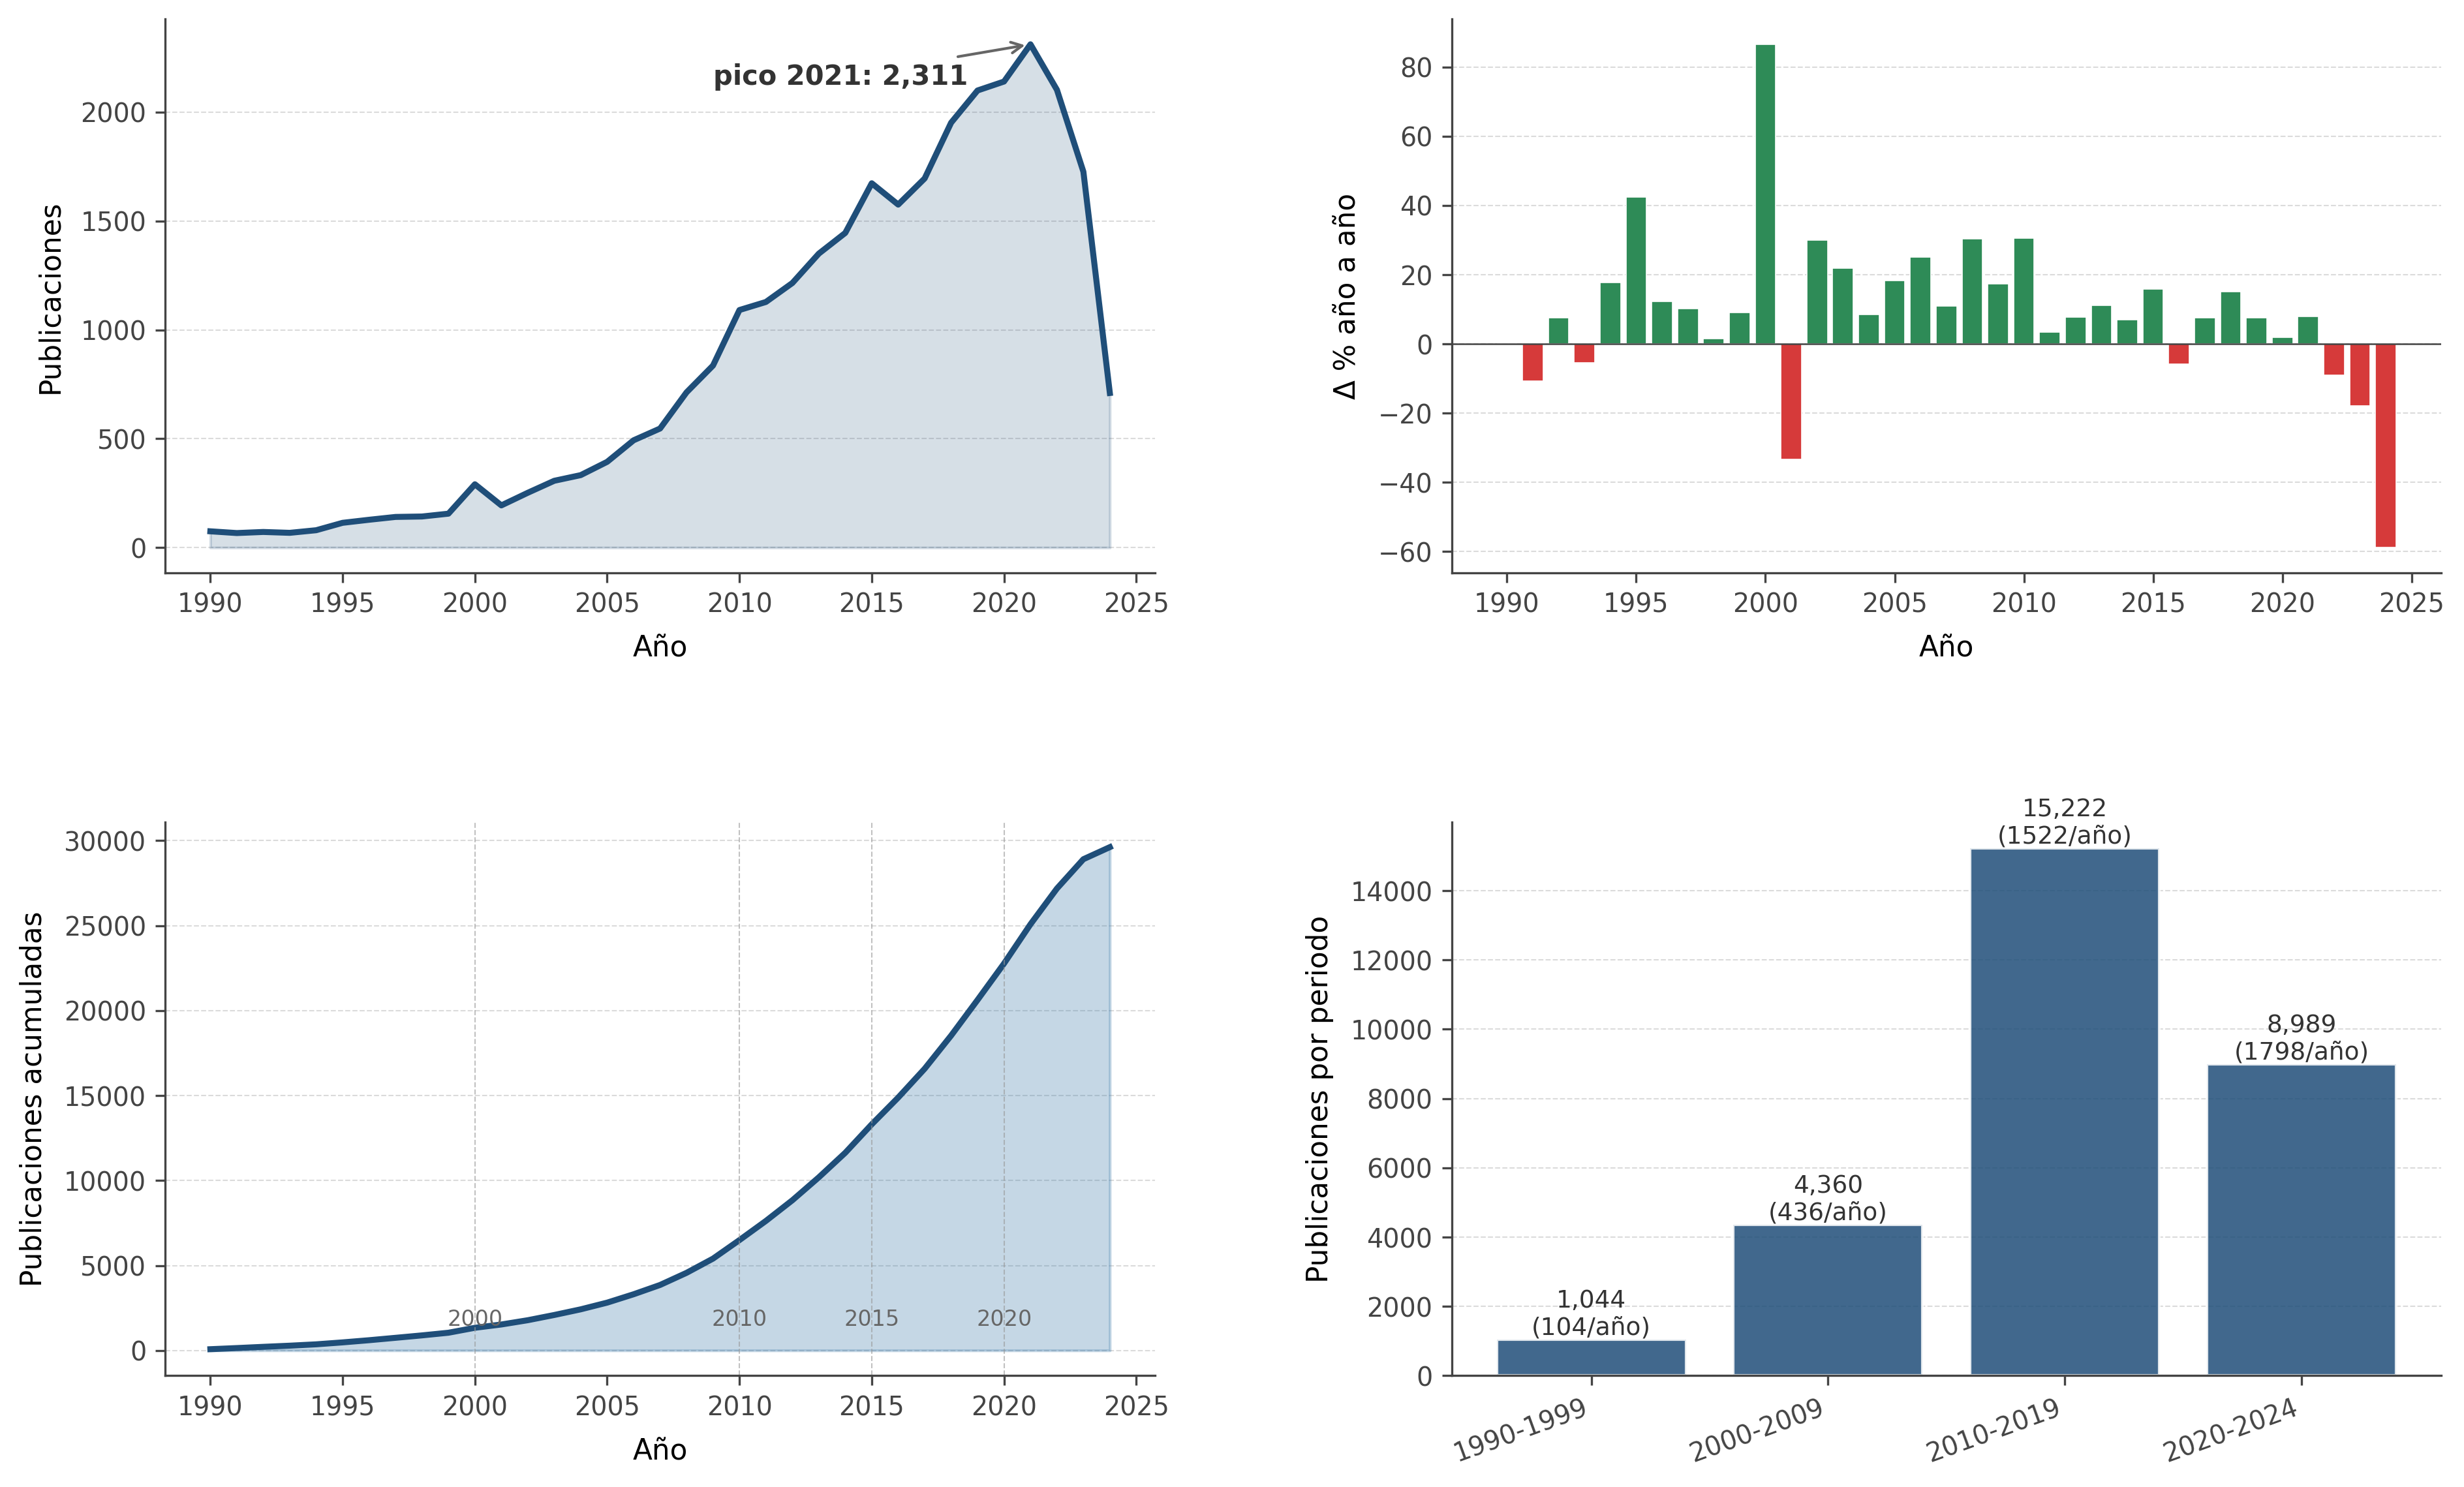
\includegraphics[width=\linewidth]{fotos/30_publication_trends.png}
\caption{Tendencia de publicación 1990--2024. \textbf{(a)} Volumen anual con pico en 2021. \textbf{(b)} Tasa de crecimiento año a año (verde positivo, rojo negativo). \textbf{(c)} Producción acumulada con hitos marcados. \textbf{(d)} Producción agregada por décadas con promedio anual.}
\label{fig:trends}
\end{figure}

La Figura~\ref{fig:trends} sintetiza el comportamiento temporal de la producción. Las observaciones clave:

\begin{table}[h]
\centering\small
\begin{tabular}{l r r r}
\toprule
\textbf{Periodo} & \textbf{Total papers} & \textbf{Promedio anual} & \textbf{Factor de crecimiento} \\
\midrule
1990--1999 & \num{1044} & 104 & --- (línea base) \\
2000--2009 & \num{4360} & 436 & $\times 4{,}2$ \\
2010--2019 & \num{15222} & \num{1522} & $\times 3{,}5$ \\
2020--2024 & \num{8989} & \good{\num{1798}} & $\times 1{,}2$ \\
\bottomrule
\end{tabular}
\caption{Producción científica UPV por décadas. El promedio anual se multiplica por $\sim 17$ entre los noventa y la década de 2020.}
\label{tab:periodos}
\end{table}

\paragraph{Crecimiento exponencial, no lineal.} La Tabla~\ref{tab:periodos} muestra que el promedio anual pasa de 104 papers (años noventa) a 1.798 papers (2020--2024): un factor de \textbf{17$\times$}. El panel (c) de la Figura~\ref{fig:trends} confirma que la curva acumulada tiene forma exponencial, no lineal. La producción acumulada total del corpus supera los \num{29000} papers con año asignado.

\paragraph{El punto de inflexión es 2005--2010.} El panel (b) revela que las mayores tasas de crecimiento interanual se concentran en 2005--2012, con un pico de \good{$+30{,}5\,\%$ en 2010}. A partir de 2015 el crecimiento se modera ($+15{,}8\,\%$) y se estabiliza: la UPV alcanza un régimen de producción \emph{maduro} de $\sim$2.000 papers/año.

\paragraph{El pico de 2021 y la caída posterior.} El máximo absoluto se alcanza en \good{2021 con 2.311 publicaciones}. La caída de 2022--2024 ($-9\,\%$ en 2022, y solo 710 papers registrados en 2024) \textbf{no debe interpretarse como pérdida de productividad}. Es un \emph{artefacto de cobertura}: las bases bibliográficas (Scopus, OpenAlex) indexan con retraso, por lo que los años más recientes aparecen sistemáticamente subrepresentados en cualquier extracción. Cualquier conclusión sobre 2022--2024 debe llevar este asterisco.

\paragraph{Implicación metodológica.} Como la producción global crece de forma exponencial, \textbf{cualquier afirmación del tipo ``los papers sobre el tema X aumentan'' es ambigua}: puede deberse a que la UPV publica más en general, no a un cambio de agenda. Por eso los análisis temáticos de la memoria principal usan series \emph{normalizadas} (porcentaje del año) y no absolutas.

% =====================================================================
\section{¿Dónde publica la UPV?}

\begin{figure}[h]
\centering
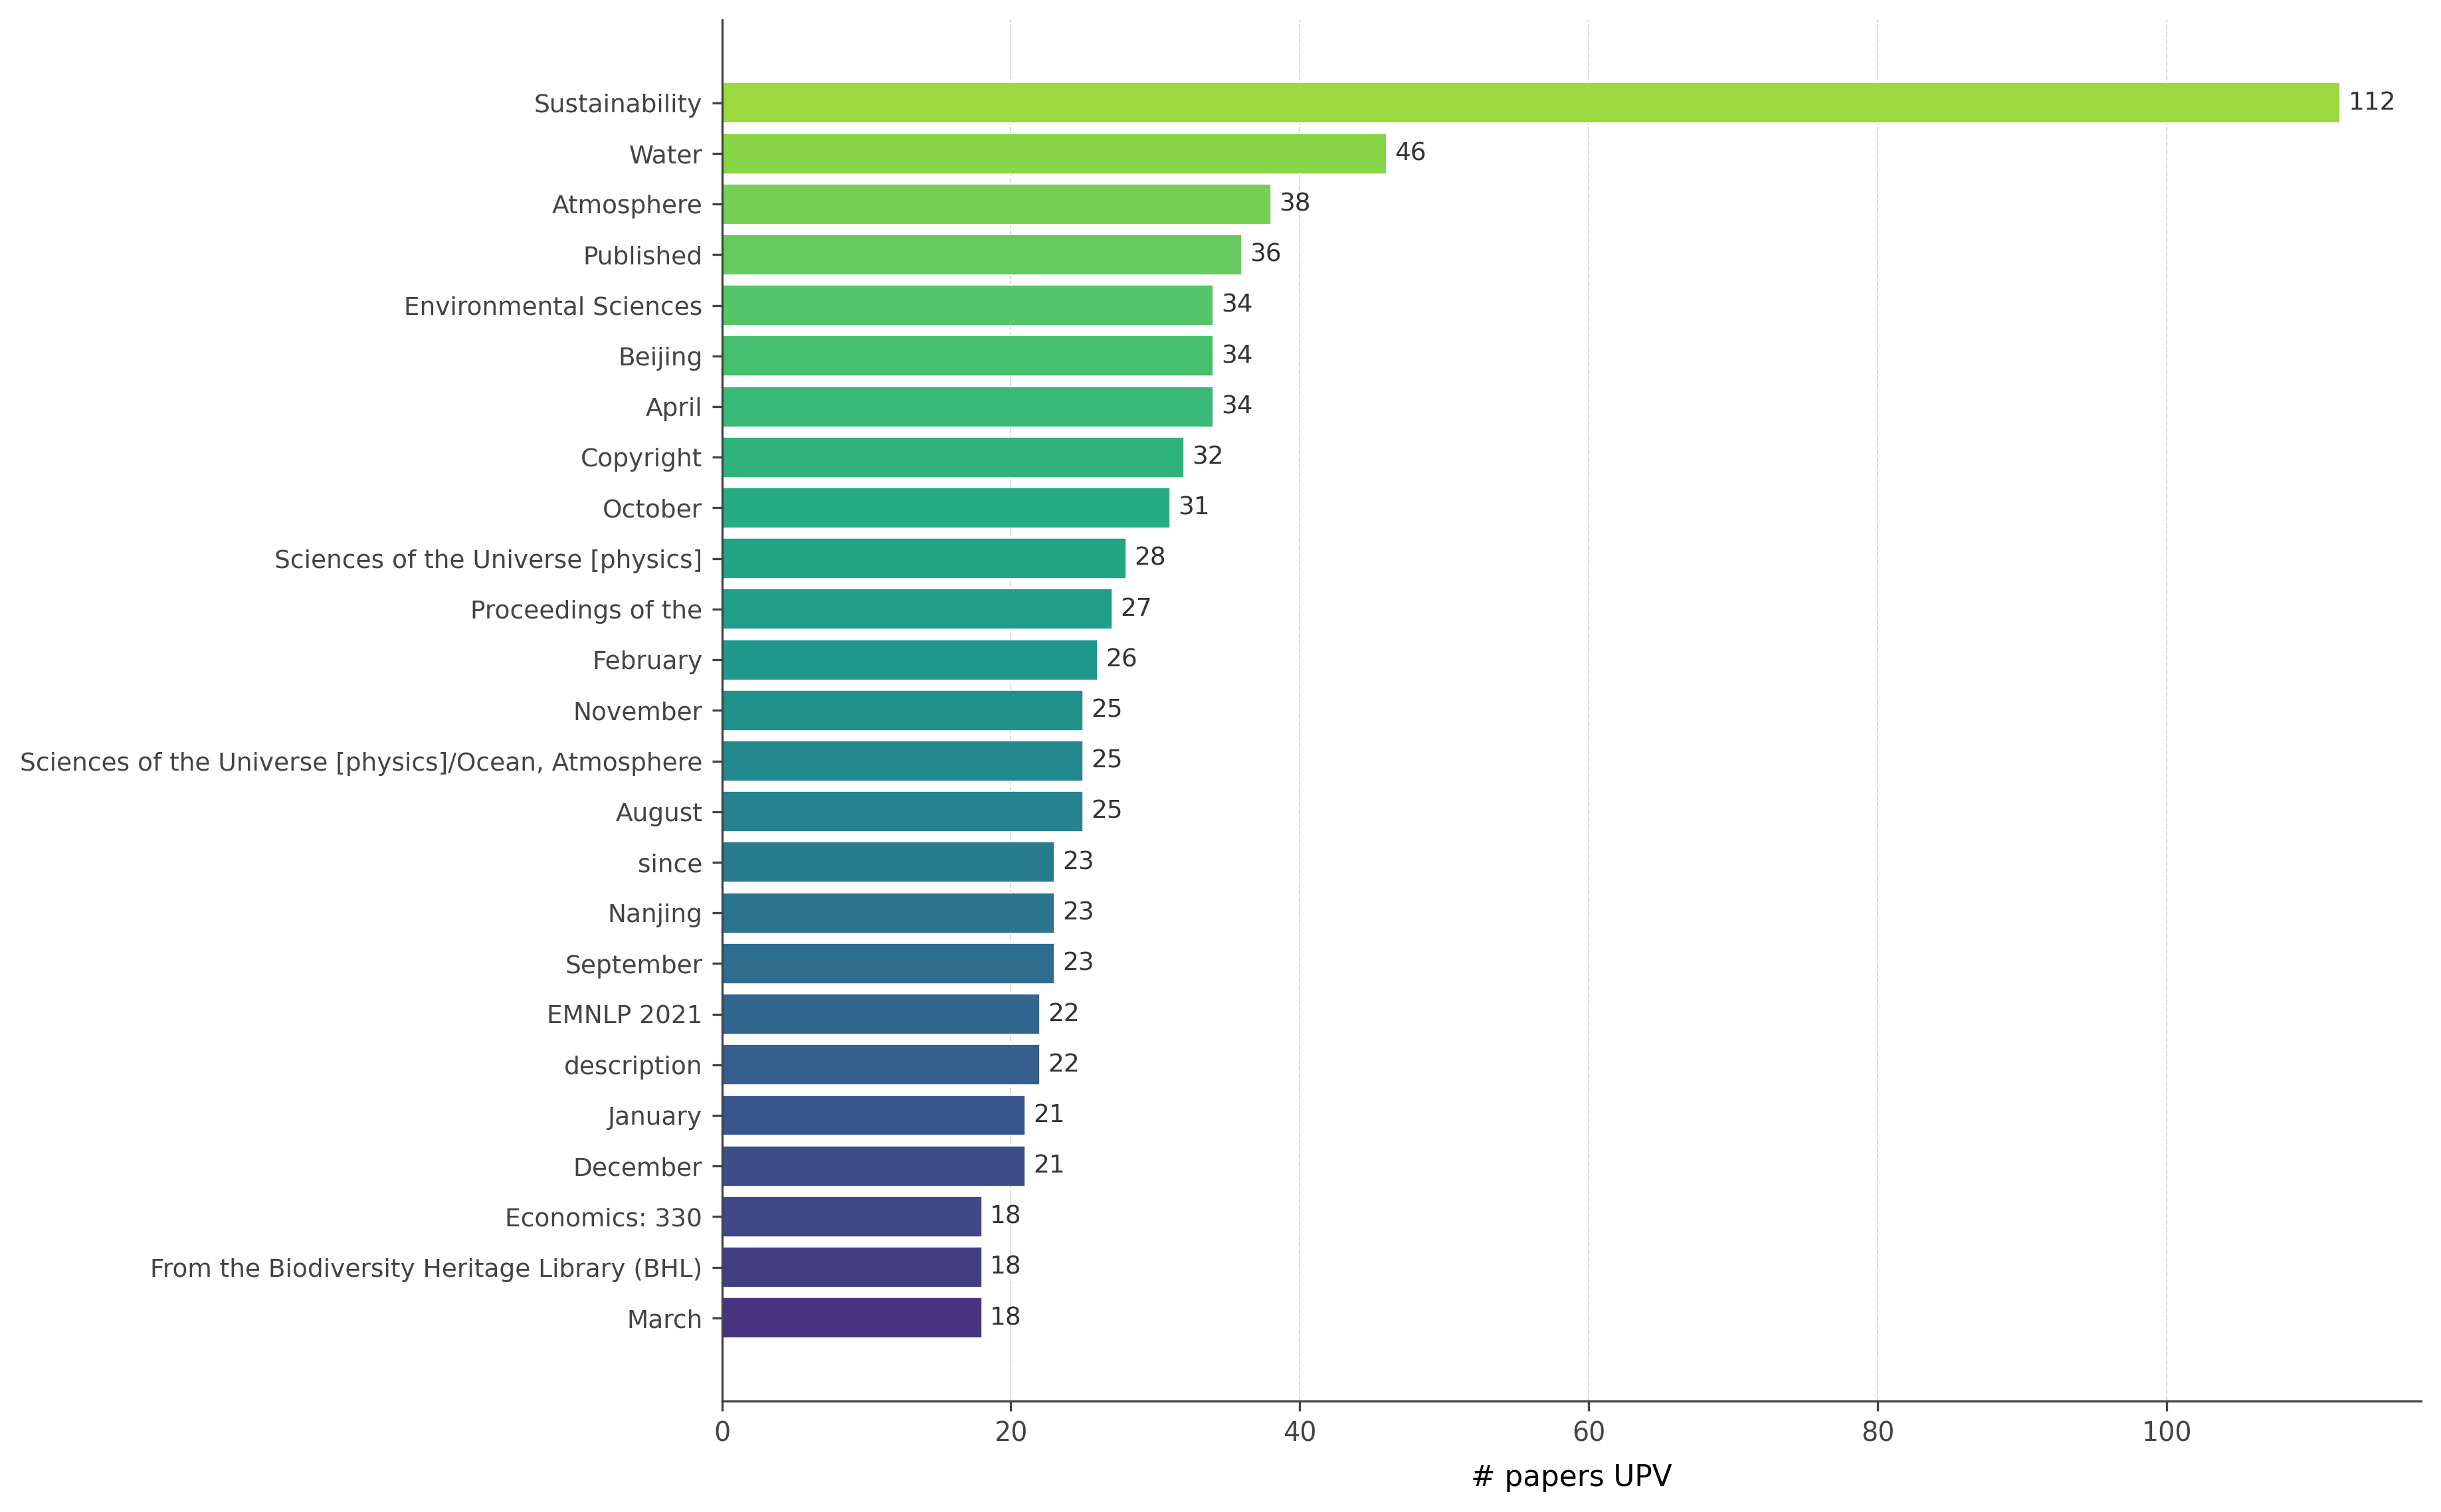
\includegraphics[width=0.82\linewidth]{fotos/31_top_journals.png}
\caption{Top 25 journals en los que publica la UPV, tras filtrar artefactos de extracción.}
\label{fig:journals}
\end{figure}

La Figura~\ref{fig:journals} muestra los 25 journals más frecuentes tras aplicar un filtro de limpieza. Tras descartar los nombres-basura, el journal más recurrente es \textbf{\emph{Sustainability}} (MDPI, 112 papers), seguido de \emph{Water} y \emph{Atmosphere} (también MDPI). El perfil revela tres rasgos:

\begin{enumerate}
\item \textbf{Preferencia por revistas \emph{open access} de gran volumen}: \emph{Sustainability}, \emph{Water}, \emph{Atmosphere}, \emph{Remote Sensing} son megajournals MDPI de acceso abierto. Es coherente con la presión institucional por publicar en abierto y con el alto throughput de estas revistas.
\item \textbf{Dispersión alta}: ningún journal concentra más del 0,4\,\% del corpus. La producción UPV está \emph{muy fragmentada} entre cientos de revistas, lo que es normal en una universidad politécnica con áreas heterogéneas.
\item \textbf{Limitación declarada}: incluso tras el filtrado, sobreviven entradas dudosas (\emph{``Published''}, \emph{``Beijing''}, nombres de meses). El campo \texttt{journal} se extrajo de PDF y arrastra ruido estructural. El ranking debe leerse como \emph{indicativo}, no exacto.
\end{enumerate}

% =====================================================================
\section{Distribución de longitud de los abstracts}

\begin{figure}[h]
\centering
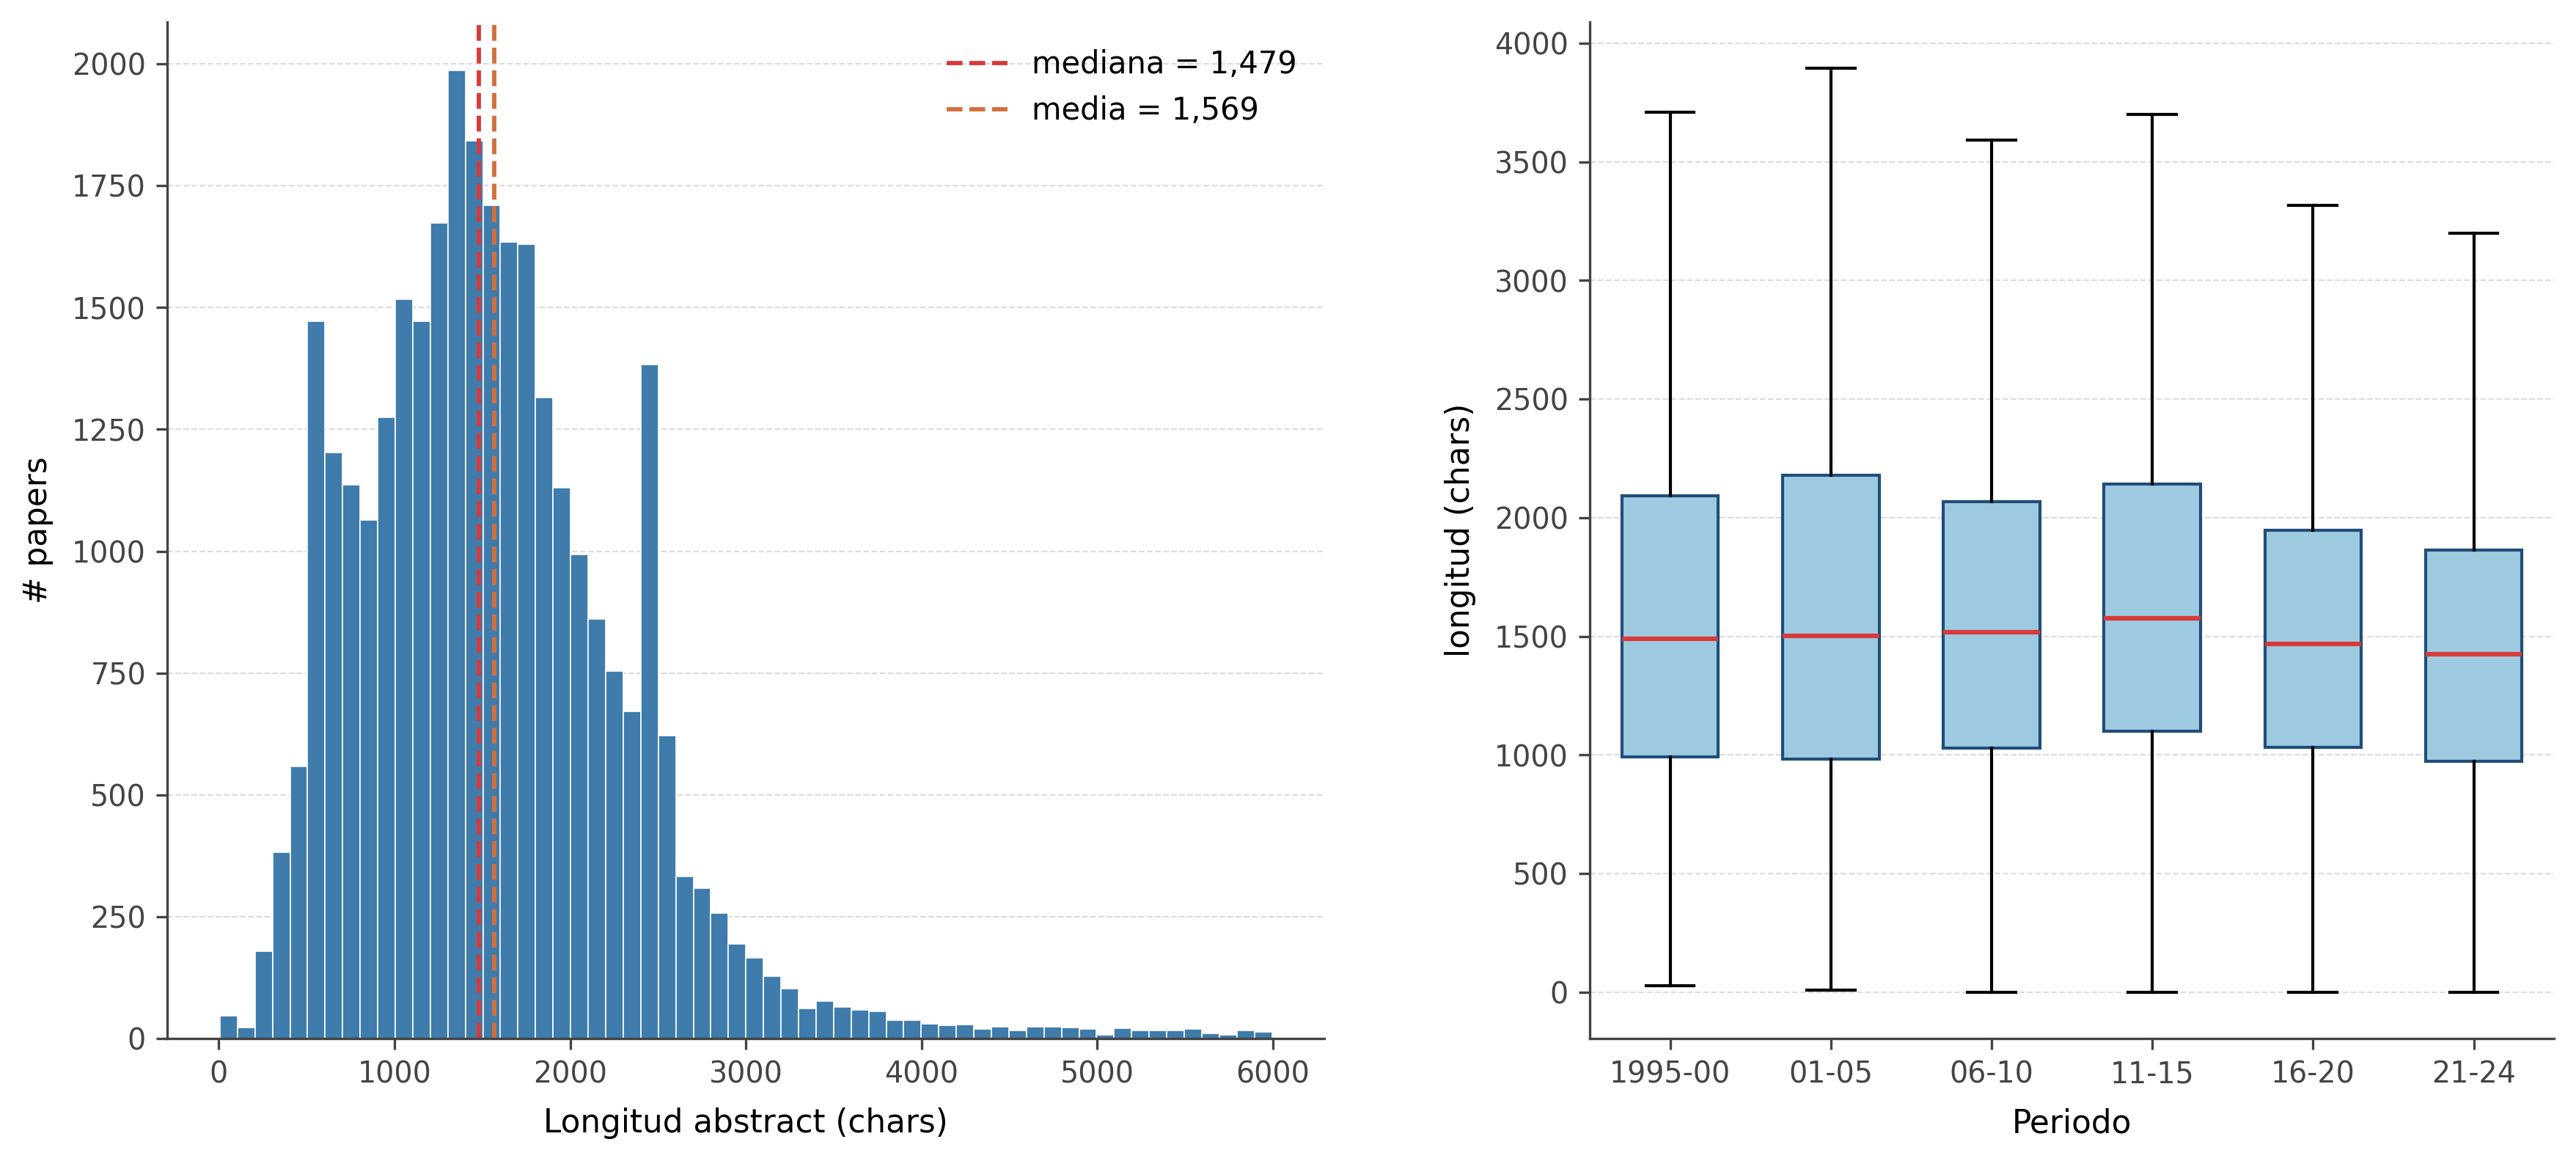
\includegraphics[width=\linewidth]{fotos/32_length_distribution.png}
\caption{Longitud de los abstracts. \textbf{(a)} Histograma global con media y mediana. \textbf{(b)} Boxplot por periodos de 5 años.}
\label{fig:length}
\end{figure}

La distribución de longitud (Figura~\ref{fig:length}) es \textbf{log-normal}, el patrón esperado para texto académico:

\begin{table}[h]
\centering\small
\begin{tabular}{l r r r r r r}
\toprule
\textbf{p10} & \textbf{p25} & \textbf{mediana} & \textbf{media} & \textbf{p75} & \textbf{p90} & \textbf{máx.} \\
\midrule
637 & \num{1028} & \good{\num{1479}} & \num{1570} & \num{1987} & \num{2489} & \num{5995} \\
\bottomrule
\end{tabular}
\caption{Estadísticos de longitud de abstract (en caracteres).}
\end{table}

\paragraph{Lectura.} La mediana de \num{1479} caracteres equivale a unos 230--250 palabras, un abstract científico típico. El que media ($\num{1570}$) supere a la mediana confirma la asimetría a la derecha: hay una cola de abstracts largos (hasta \num{5995} caracteres) que tira de la media. El panel (b) muestra que la longitud mediana es \textbf{estable a lo largo de las décadas}: los abstracts no se han alargado ni acortado sistemáticamente, lo que da homogeneidad al corpus para análisis NLP.

\paragraph{Relevancia para el modelado.} La p90 de \num{2489} caracteres ($\approx$ 400 palabras $\approx$ 520 tokens) justifica el \texttt{max\_length=256} usado en los transformers: trunca solo el 10\,\% más largo del corpus, y normalmente la parte truncada es metodología secundaria, no la tesis central del abstract.

% =====================================================================
\section{¿De qué habla la UPV? Vocabulario más frecuente}

\begin{figure}[h]
\centering
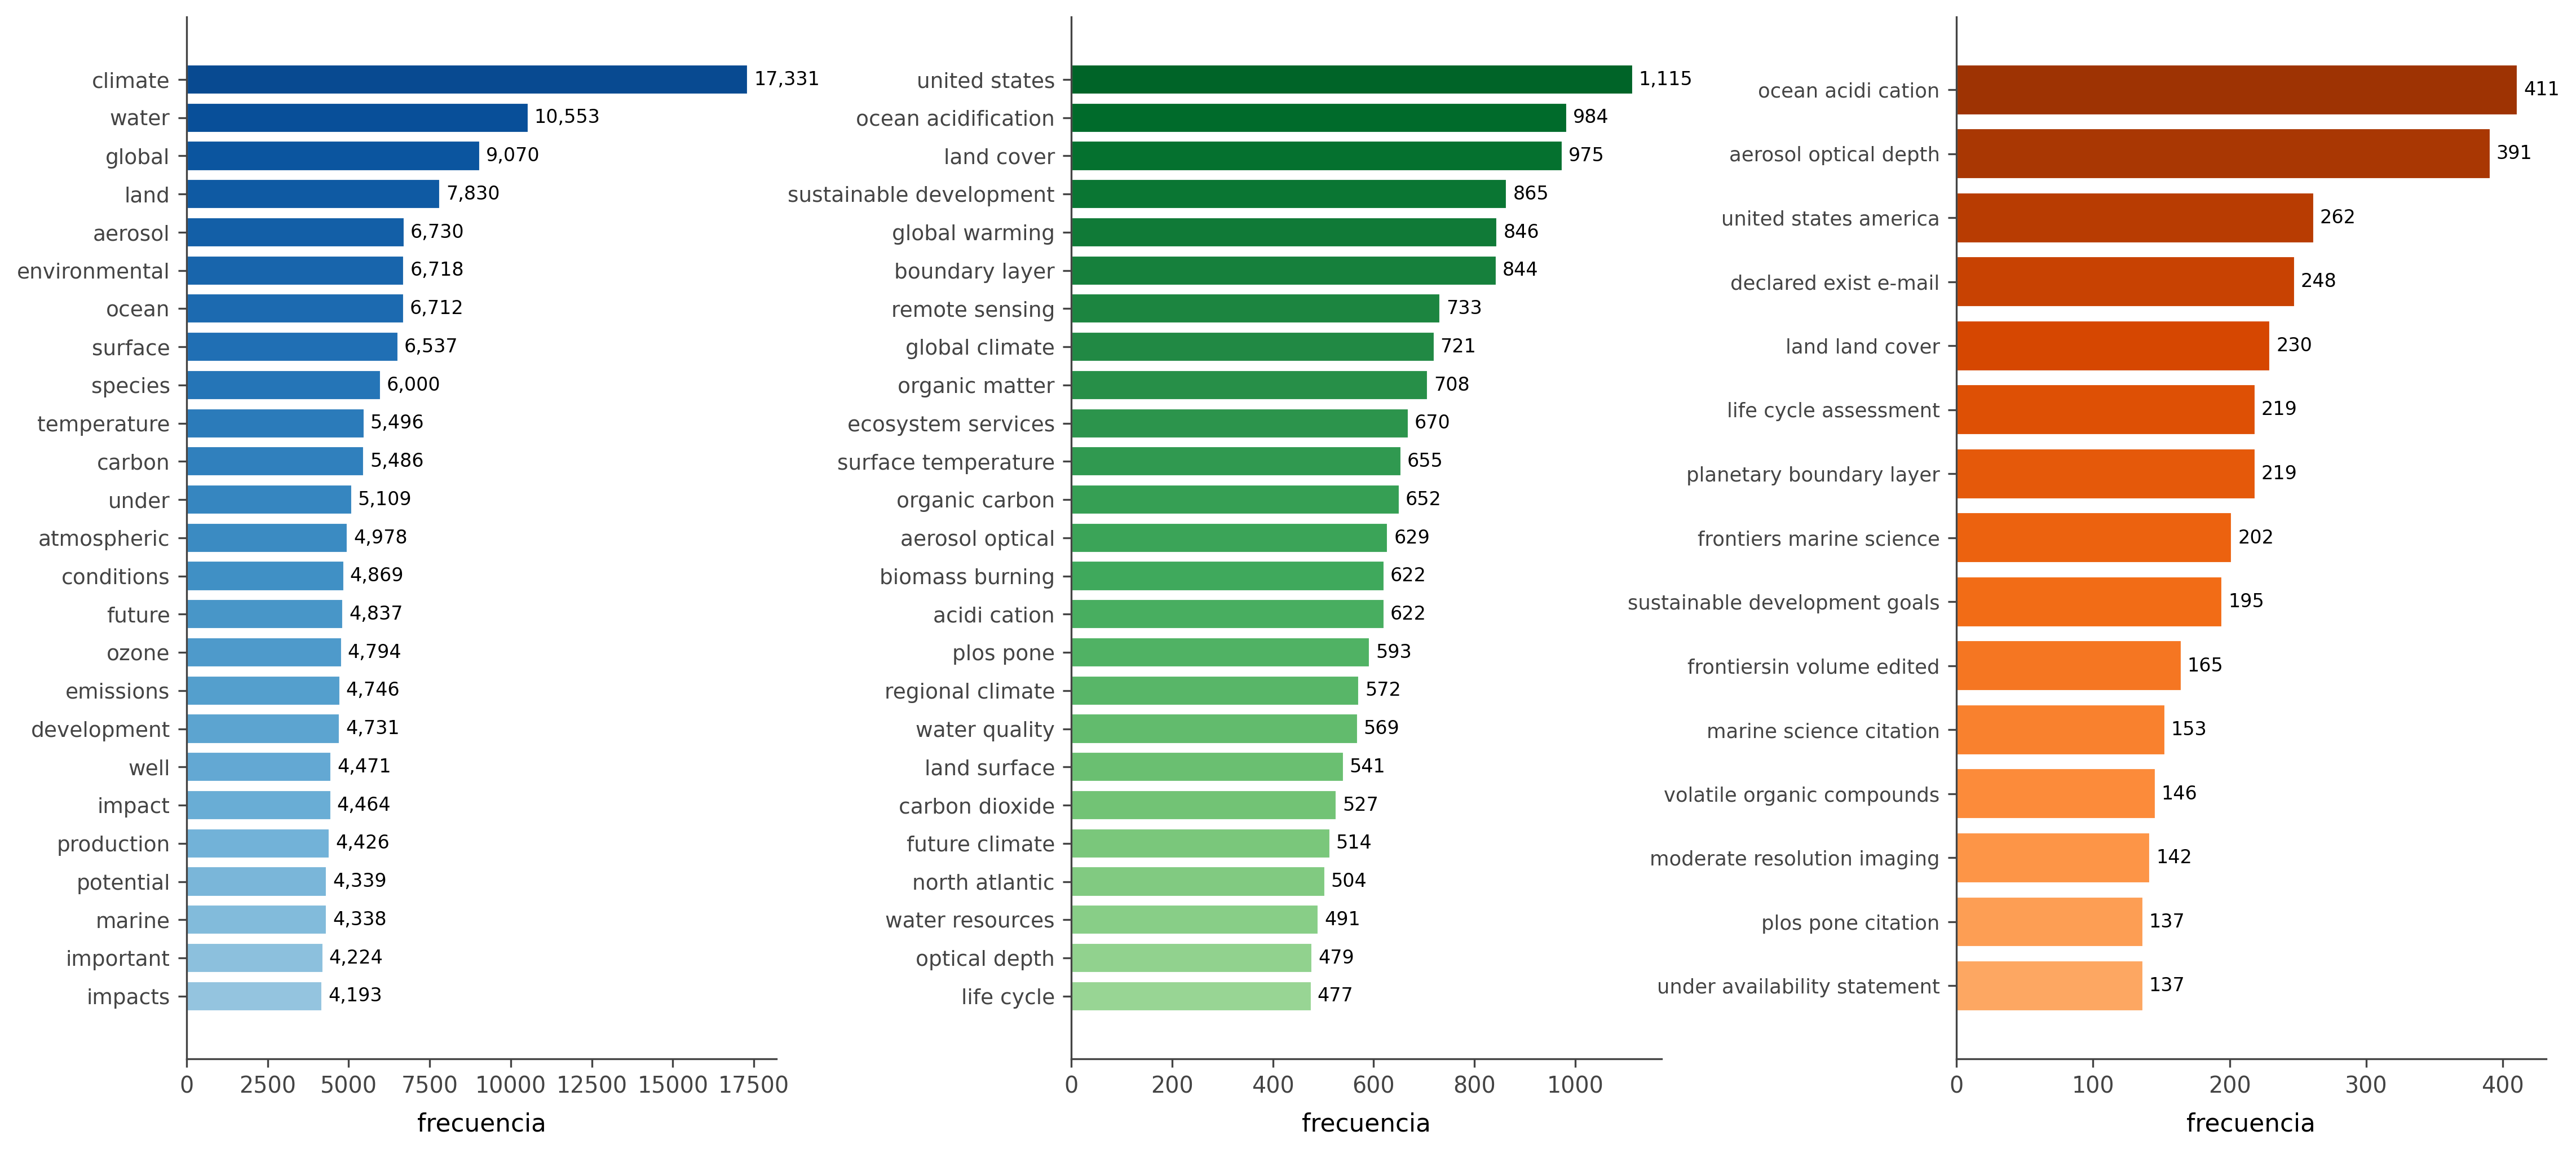
\includegraphics[width=\linewidth]{fotos/33_top_ngrams.png}
\caption{Vocabulario más frecuente: unigramas, bigramas y trigramas (muestra de 20.000 abstracts, tras eliminar stopwords y boilerplate editorial).}
\label{fig:ngrams}
\end{figure}

\begin{figure}[h]
\centering
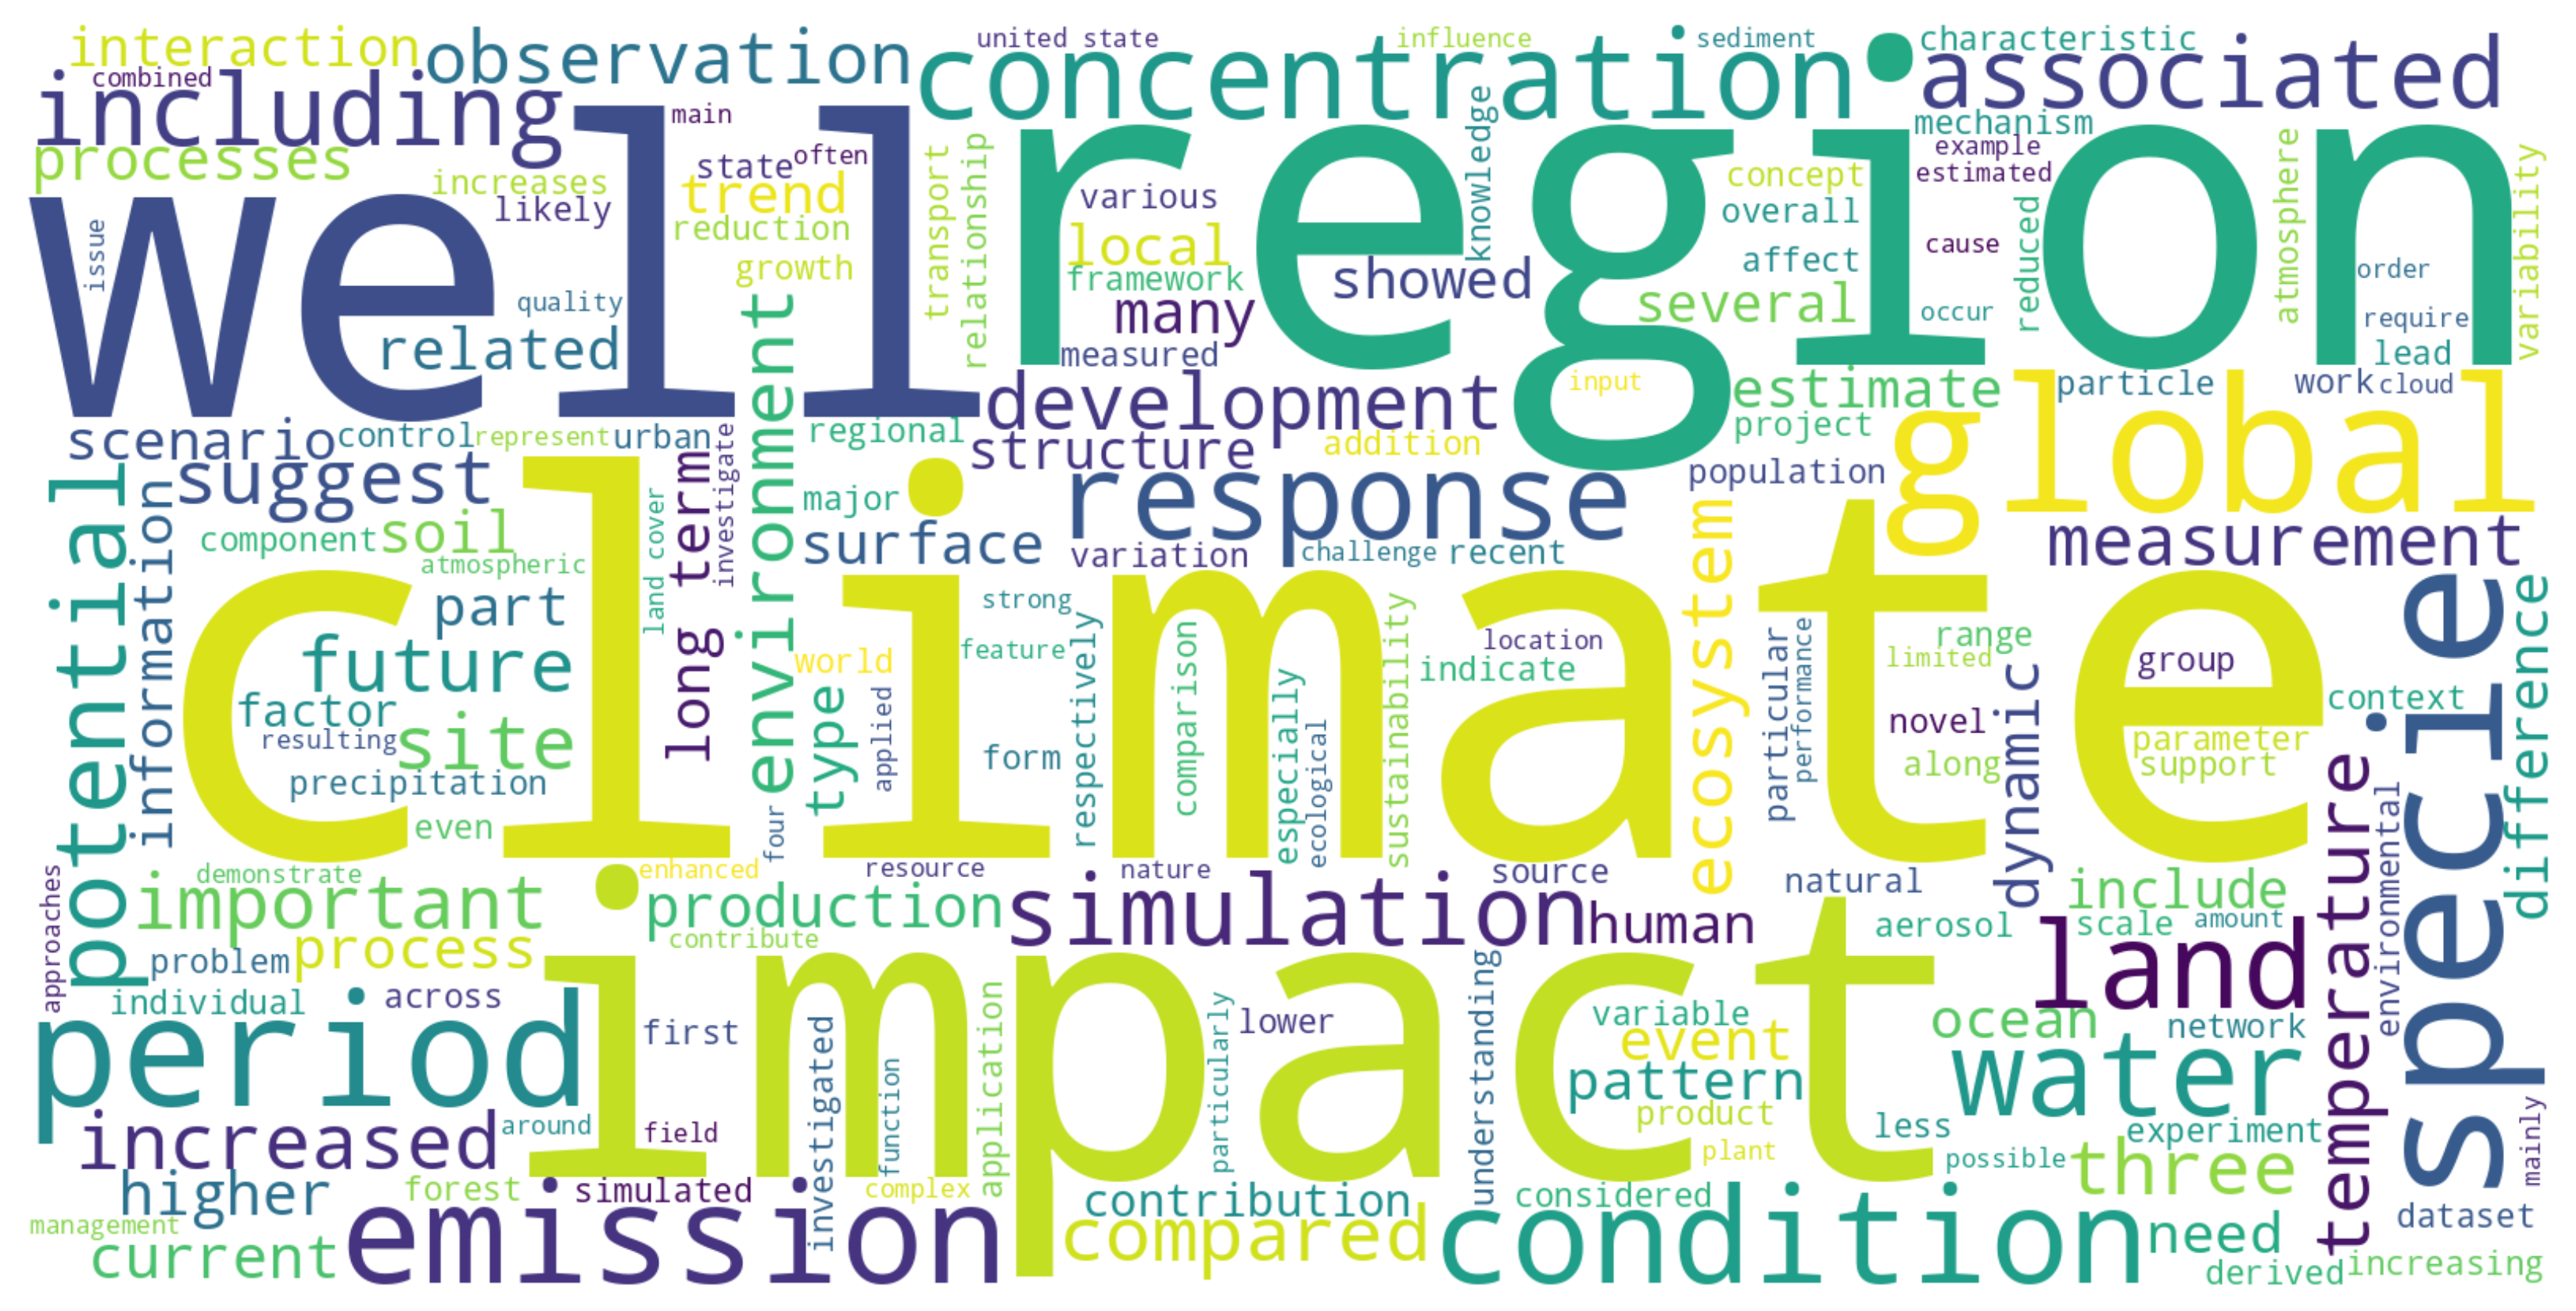
\includegraphics[width=0.82\linewidth]{fotos/35_wordcloud_global.png}
\caption{Wordcloud global del corpus UPV.}
\label{fig:wordcloud}
\end{figure}

La Figura~\ref{fig:ngrams} y el wordcloud (Figura~\ref{fig:wordcloud}) muestran el vocabulario del corpus tras un preprocesado exigente: eliminación de \emph{stopwords} genéricas, de boilerplate editorial (\emph{creative commons}, \emph{copernicus publications}, nombres de meses) y reparación de ligaduras rotas.

\begin{table}[h]
\centering\small
\begin{tabularx}{\linewidth}{X X}
\toprule
\textbf{Top unigramas} & \textbf{Top bigramas} \\
\midrule
climate (\num{17331}), water (\num{10553}), global (\num{9070}), land (\num{7830}), aerosol (\num{6730}), environmental (\num{6718}), ocean (\num{6712}), surface (\num{6537}), species (\num{6000}), temperature (\num{5496}), carbon (\num{5486}) &
united states (\num{1115}), ocean acidification (984), land cover (975), sustainable development (865), global warming (846), boundary layer (844), remote sensing (733), global climate (721), organic matter (708), ecosystem services (670) \\
\bottomrule
\end{tabularx}
\caption{Vocabulario más frecuente del corpus (frecuencias sobre la muestra).}
\label{tab:vocab}
\end{table}

\paragraph{Lectura interpretativa.} El vocabulario confirma de forma independiente la firma temática detectada en la memoria PB:

\begin{itemize}
\item \textbf{Clima domina}: ``climate'' es el unigrama más frecuente con diferencia (\num{17331}), y ``climate change'' / ``global warming'' / ``global climate'' encabezan los bigramas. Coincide con que PB1 (Climate Change) sea el PB dominante.
\item \textbf{Agua y suelo en segundo plano}: ``water'' (2º unigrama) y ``land'' / ``land cover'' confirman el peso de PB5 (Freshwater) y PB6 (Land-System).
\item \textbf{Atmósfera}: ``aerosol'', ``surface'', ``temperature'', ``boundary layer'' reflejan PB9 (Aerosol Loading) y la fuerte línea de física atmosférica.
\item \textbf{Vocabulario metodológico}: ``remote sensing'', ``ecosystem services'' indican \emph{cómo} se hace la investigación (teledetección, valoración de servicios ecosistémicos).
\end{itemize}

\paragraph{Limitación de los trigramas.} Los trigramas son el nivel más contaminado: pese al filtrado, sobreviven fragmentos de declaraciones de conflicto de interés y de financiación (\emph{``without written consent''}, \emph{``declared exist''}). Los trigramas \emph{legítimos} que sí emergen son informativos --- \emph{``aerosol optical depth''}, \emph{``life cycle assessment''}, \emph{``planetary boundary layer''}, \emph{``sustainable development goals''} --- pero el ranking de trigramas debe leerse con más cautela que el de unigramas/bigramas.

% =====================================================================
\section{Vocabulario emergente: ¿qué temas son nuevos?}

\begin{figure}[h]
\centering
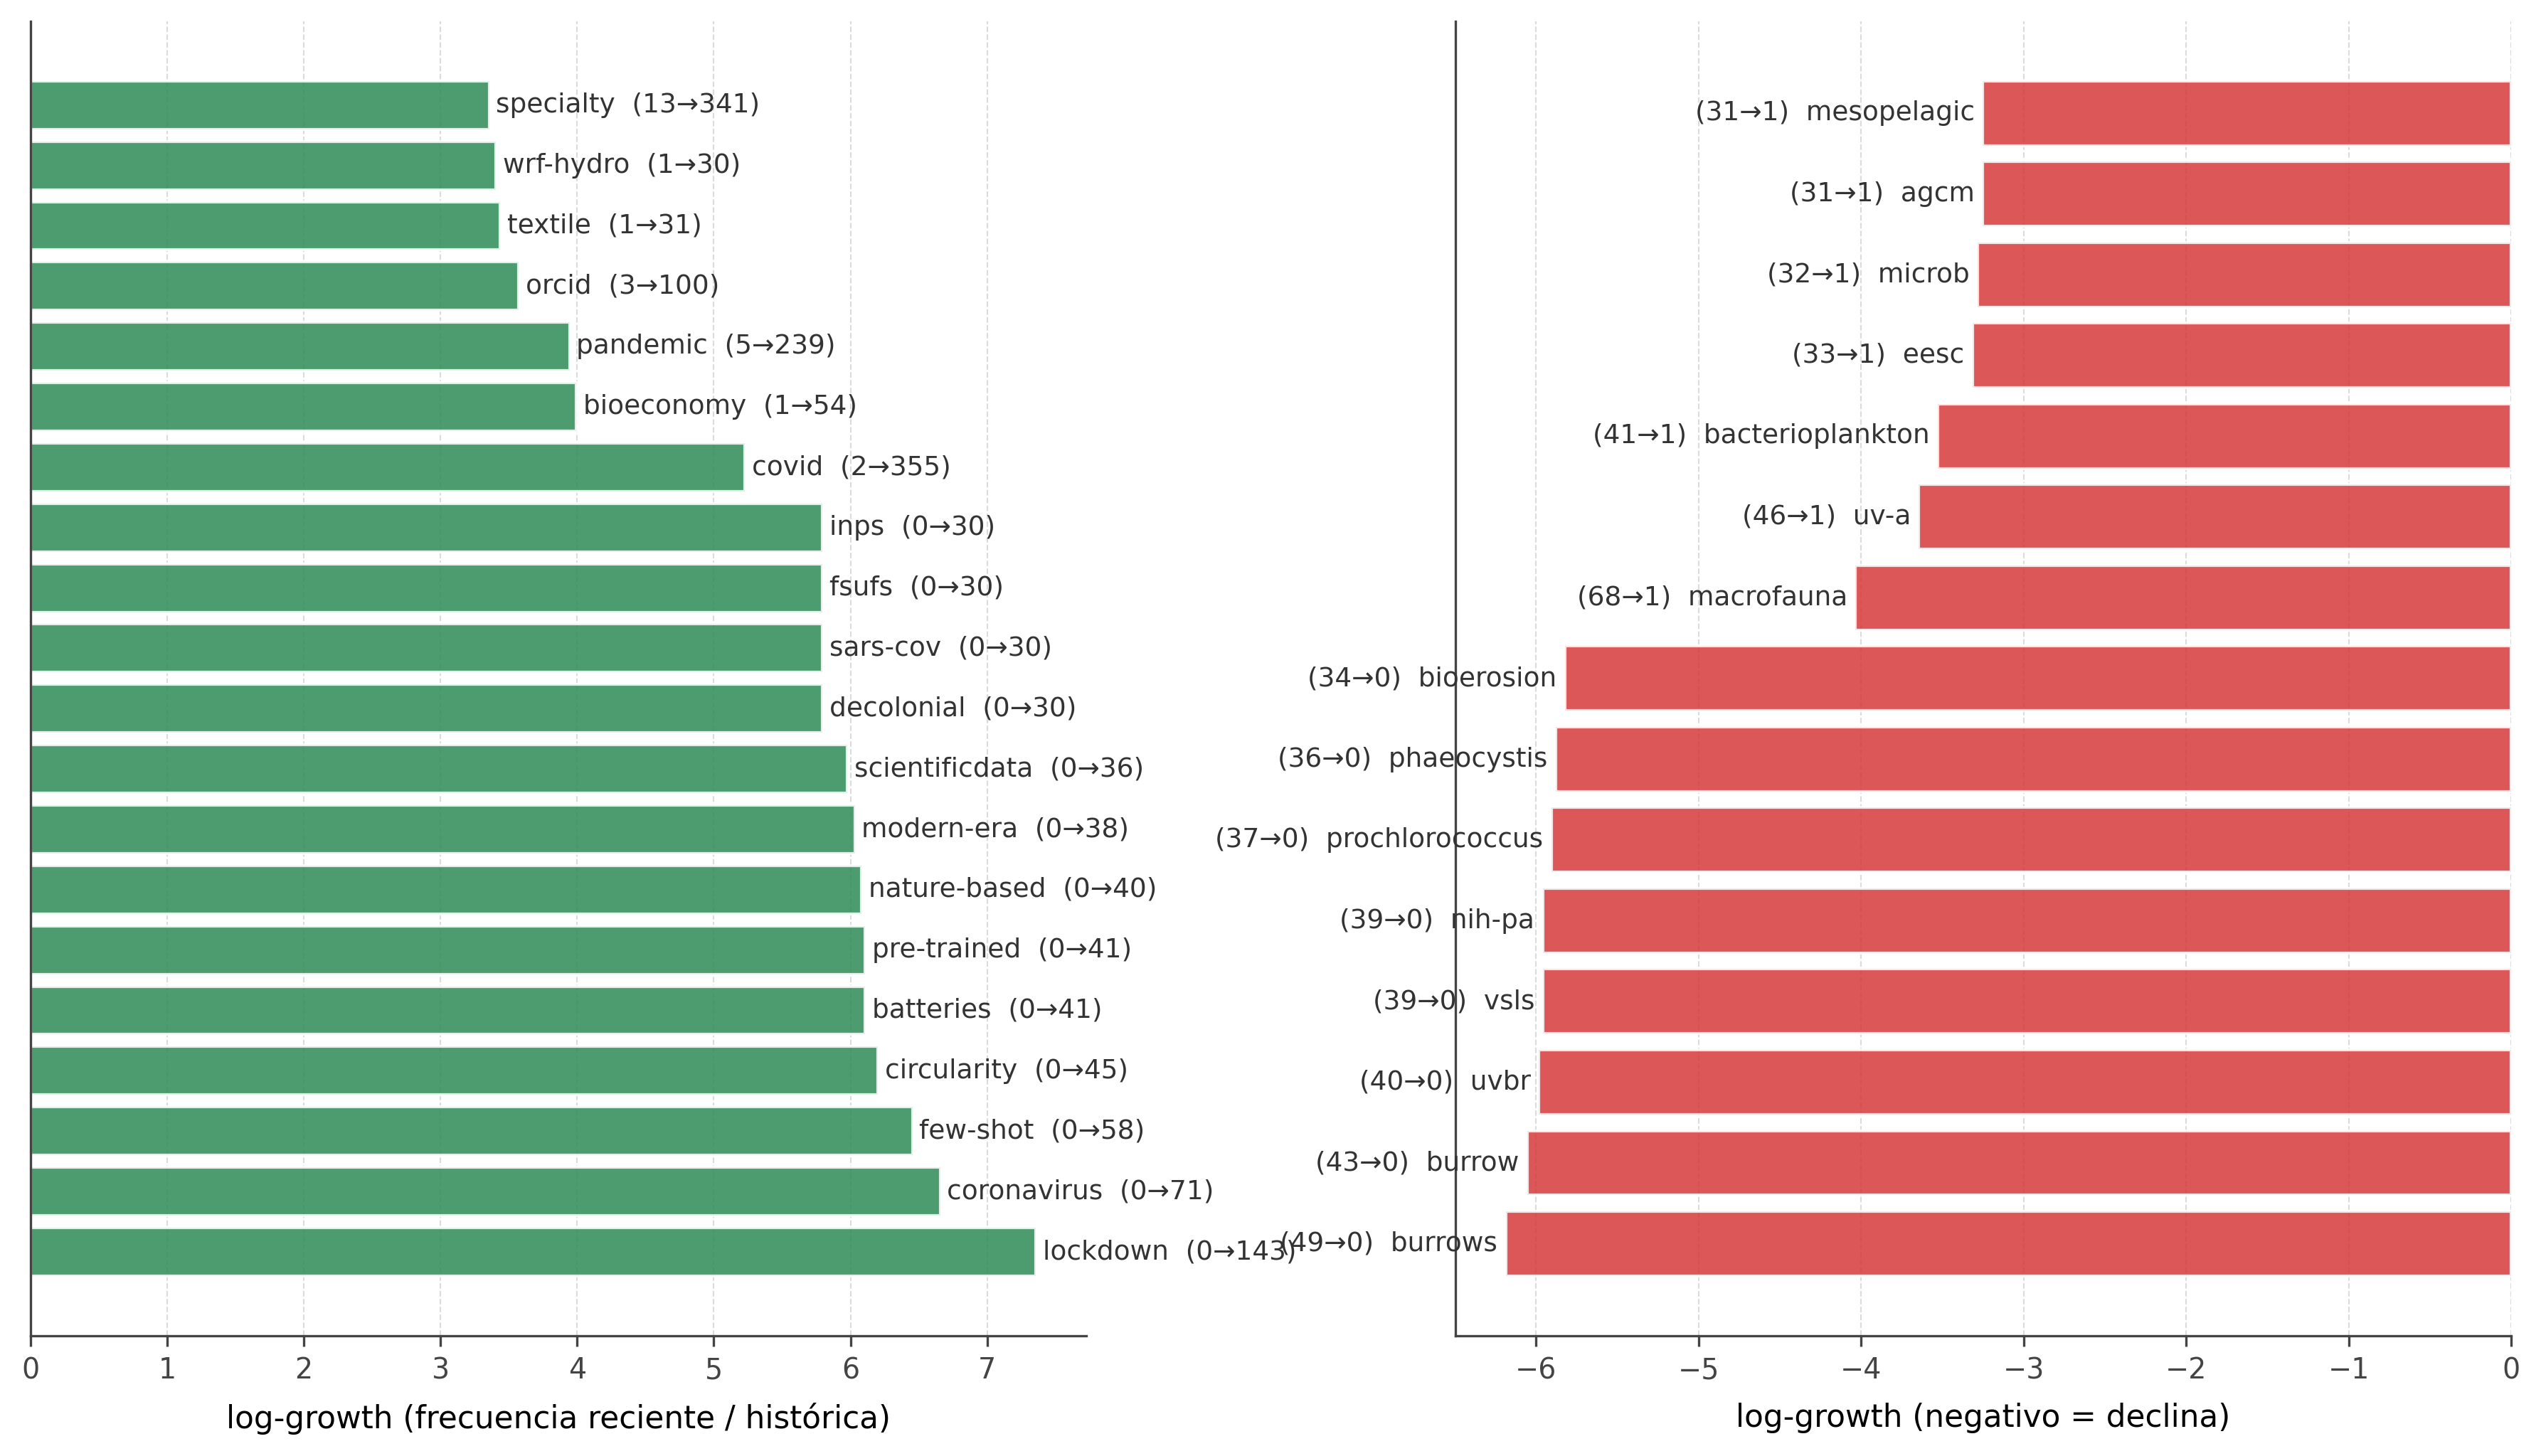
\includegraphics[width=\linewidth]{fotos/34_emerging_terms.png}
\caption{Vocabulario emergente vs en declive. Se compara la frecuencia relativa de cada término entre los abstracts $\leq$2015 y los $\geq$2020. \textbf{(a)} Términos que más crecen. \textbf{(b)} Términos en declive.}
\label{fig:emerging}
\end{figure}

La Figura~\ref{fig:emerging} aplica una métrica de \emph{log-growth}: para cada término, $\ln(\text{freq}_{\geq 2020} / \text{freq}_{\leq 2015})$. Un valor positivo grande señala un término que era raro o inexistente antes de 2015 y se ha vuelto frecuente. Es la forma rigurosa de detectar \textbf{cambios de agenda investigadora}.

\paragraph{Tres olas de vocabulario emergente.} Los términos que más crecen se agrupan en tres familias temáticas reconocibles:

\begin{enumerate}
\item \textbf{Ola pandémica}: \emph{lockdown}, \emph{coronavirus}, \emph{covid}, \emph{sars-cov}. La pandemia de 2020 generó una línea de investigación sobre su efecto en la calidad del aire, en los aerosoles y en la movilidad --- temas que tocan directamente PB9.
\item \textbf{Ola de economía circular y transición}: \emph{circularity}, \emph{batteries}, \emph{nature-based} (soluciones basadas en la naturaleza). Refleja la incorporación de la agenda de transición ecológica y economía circular en la investigación UPV reciente.
\item \textbf{Ola de Machine Learning}: \emph{few-shot}, \emph{pre-trained}. El propio vocabulario del aprendizaje automático moderno irrumpe en los abstracts, señal de que la UPV aplica cada vez más NLP/ML a problemas ambientales --- exactamente lo que este proyecto ejemplifica.
\end{enumerate}

\paragraph{Vocabulario en declive.} En el lado opuesto, términos como \emph{vsls} (\emph{very short-lived substances}, química de ozono), \emph{prochlorococcus} o \emph{phaeocystis} (taxones de plancton) pierden peso relativo. No significa que la UPV abandone esos temas; significa que el corpus reciente se diversifica y esos nichos muy específicos se diluyen proporcionalmente.

\paragraph{Lectura crítica.} El análisis de términos emergentes es la herramienta más potente de este AED porque \textbf{detecta agenda, no volumen}. Confirma que la UPV es una institución científica \emph{reactiva a los acontecimientos globales}: la pandemia, la agenda de transición ecológica y la revolución del ML aparecen en su vocabulario con un retraso de 2--3 años, coherente con los tiempos de revisión y publicación.

% =====================================================================
\section{Fuentes, metadatos y coautoría}

\begin{figure}[h]
\centering
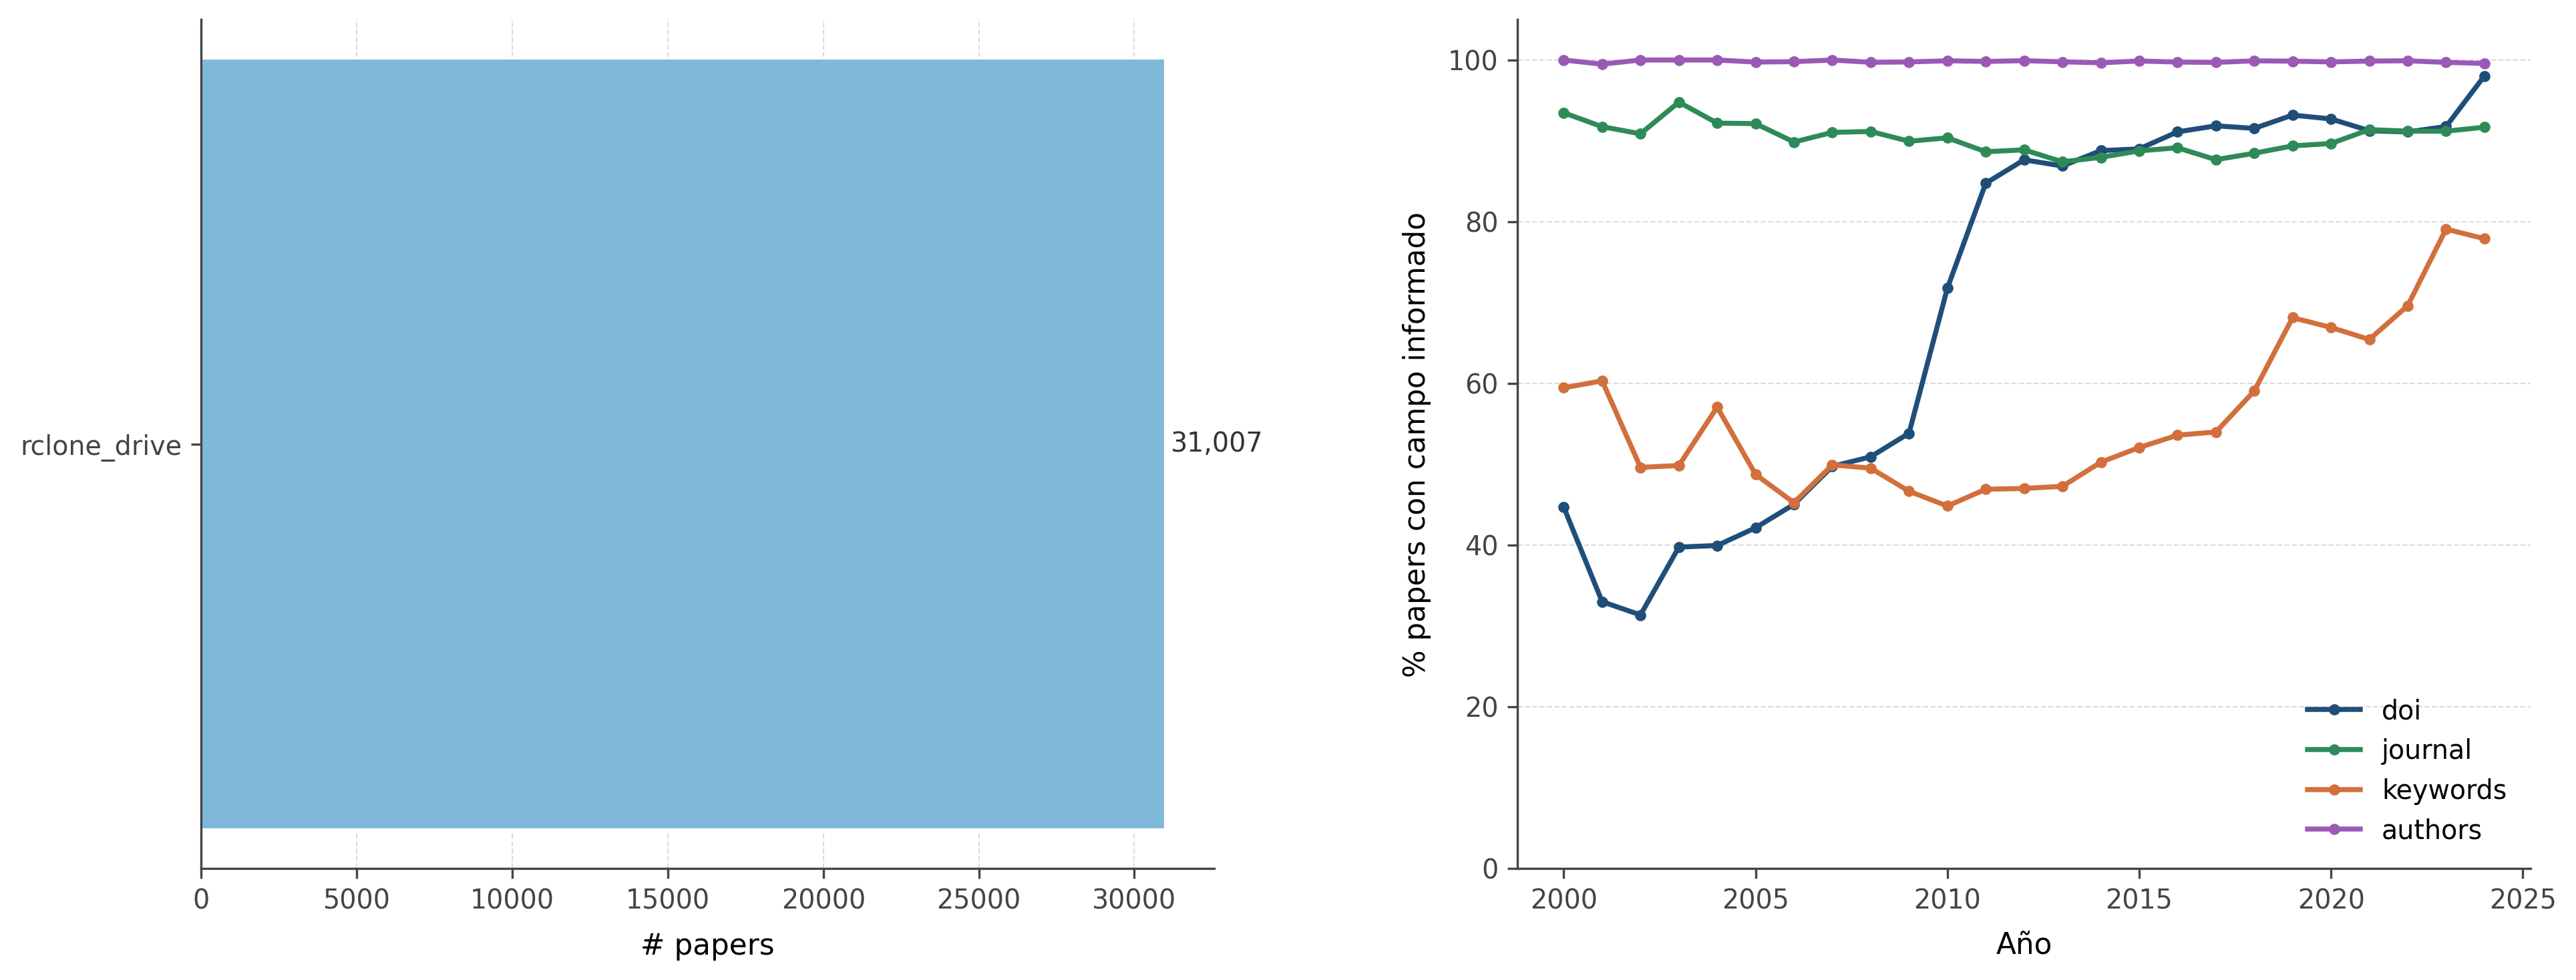
\includegraphics[width=\linewidth]{fotos/36_sources_completeness.png}
\caption{\textbf{(a)} Fuentes del corpus. \textbf{(b)} Completitud de metadatos por año.}
\label{fig:sources}
\end{figure}

\begin{figure}[h]
\centering
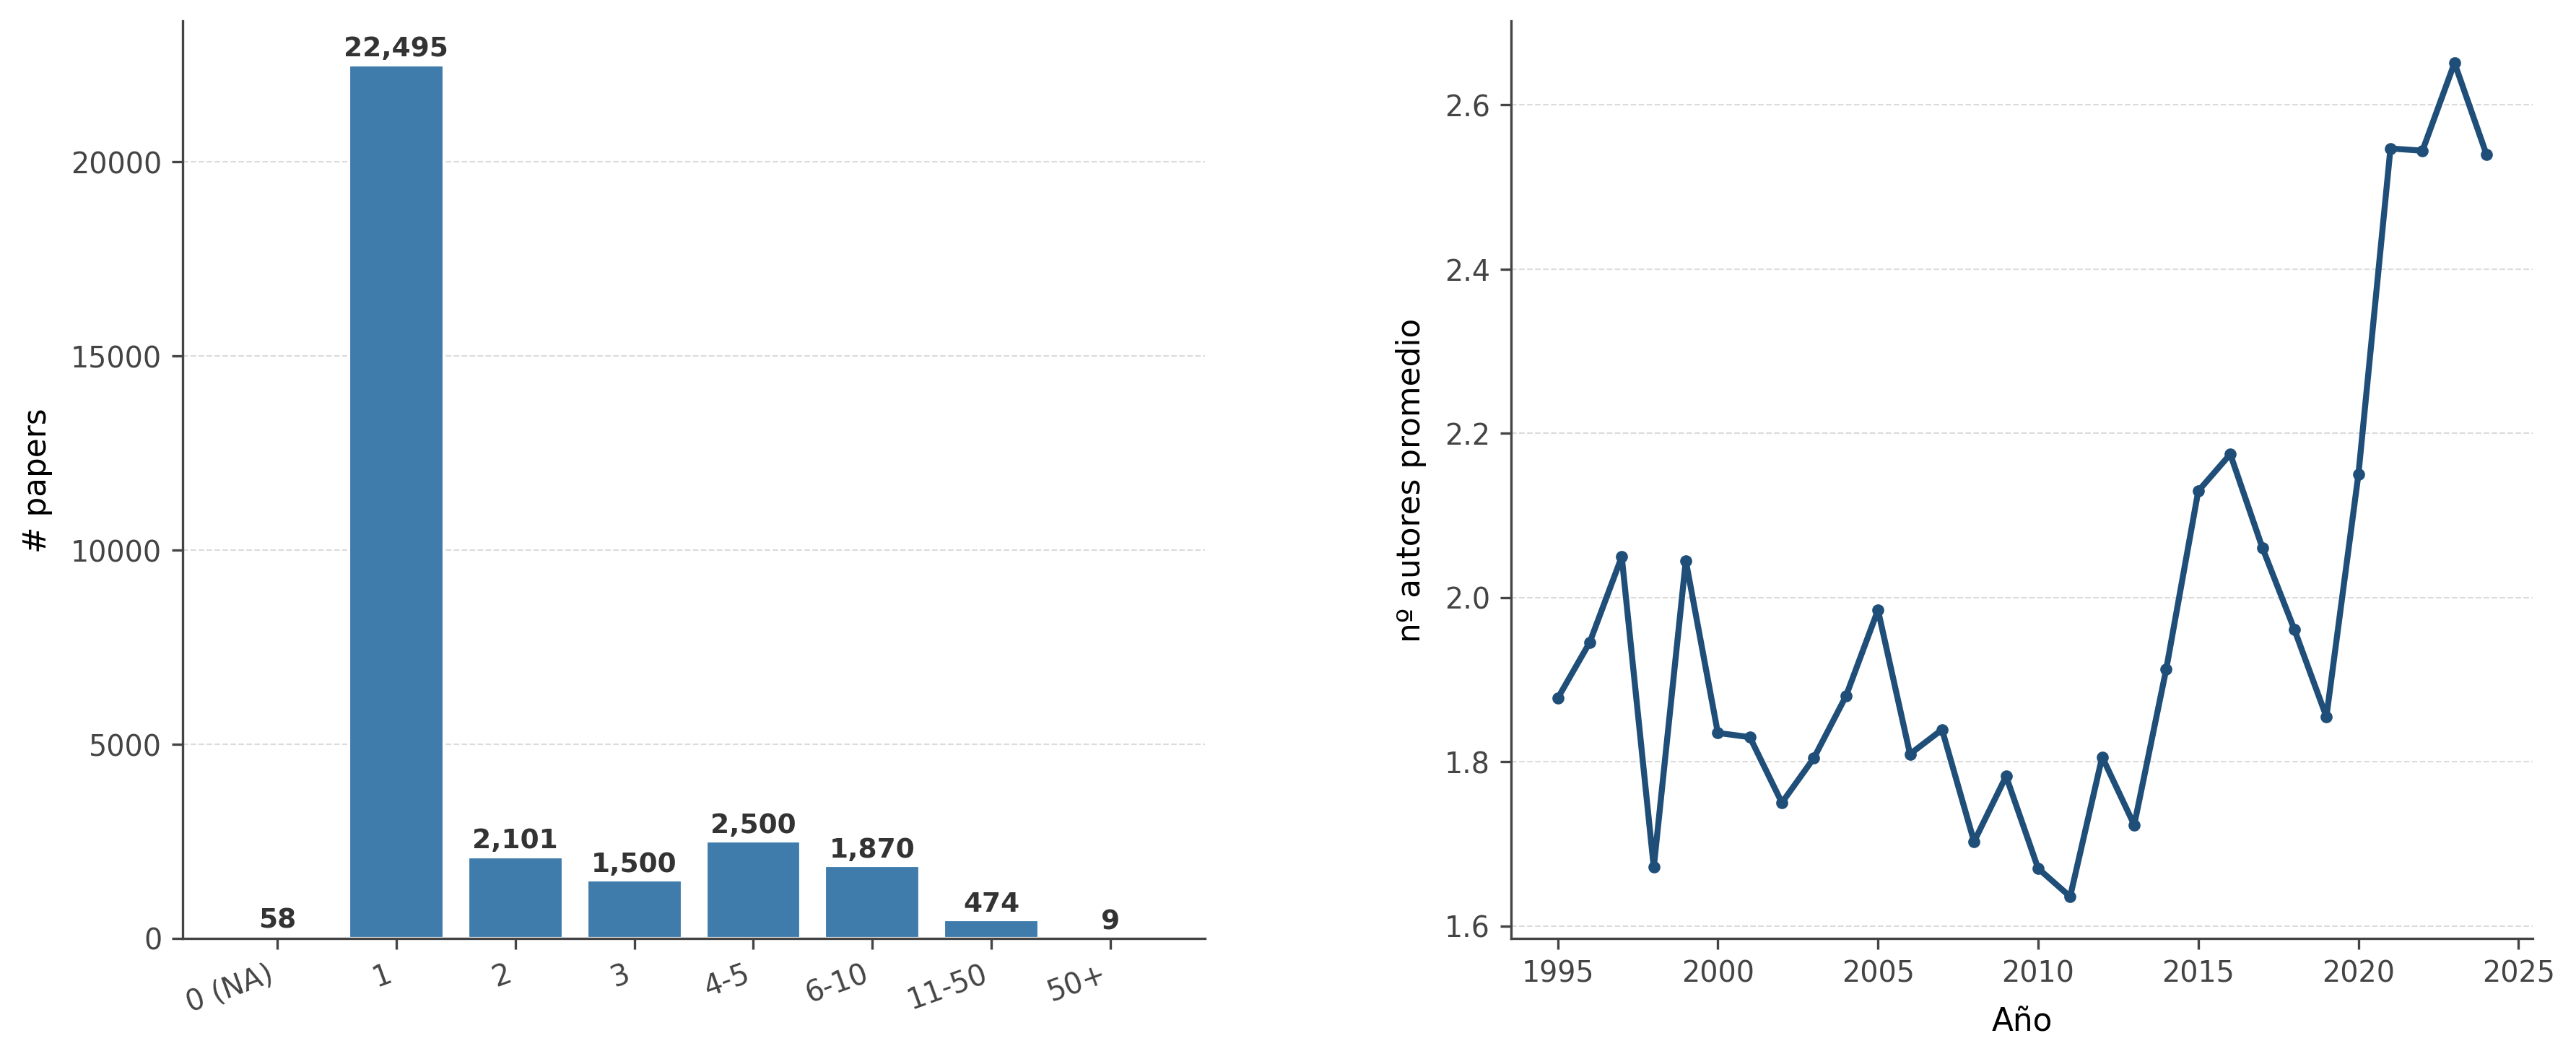
\includegraphics[width=\linewidth]{fotos/37_authorship_collaboration.png}
\caption{Coautoría. \textbf{(a)} Distribución del nº de autores por paper. \textbf{(b)} Evolución del tamaño medio de equipo.}
\label{fig:authors}
\end{figure}

\paragraph{Fuentes.} El corpus consolidado se sirve íntegramente vía \texttt{rclone\_drive} (un único almacenamiento UPV que integra upstream las descargas de Scopus + OpenAlex). La completitud de metadatos por año (Figura~\ref{fig:sources}b) muestra que \texttt{journal} y \texttt{authors} están bien informados en los años recientes, mientras que \texttt{doi} y \texttt{keywords} tienen lagunas mayores --- el \texttt{doi} es especialmente incompleto en los registros antiguos, un patrón conocido de OpenAlex.

\paragraph{Coautoría: cifra no fiable.} La Figura~\ref{fig:authors} debe leerse con la máxima cautela. La distribución indica que la mayoría de los papers tendría \emph{un solo autor}, lo cual es \textbf{científicamente inverosímil} para un corpus de earth science (donde lo normal son 3--8 coautores). La causa es técnica: el campo \texttt{authors} no se separa de forma consistente (mezcla de separadores ``;'', ``,'' y formatos heterogéneos por fuente). Por tanto, \textbf{la cifra de coautoría de este AED no es un resultado válido}; se incluye solo para documentar la limitación y motivar un trabajo futuro de re-parsing del campo \texttt{authors}.

% =====================================================================
\section{Calidad de datos: lo que el AED ha tenido que corregir}\label{sec:calidad}

Un AED honesto documenta el ruido que ha tenido que limpiar. Las tres correcciones aplicadas:

\begin{table}[h]
\centering\small
\begin{tabularx}{\linewidth}{l X}
\toprule
\textbf{Problema} & \textbf{Corrección aplicada} \\
\midrule
Boilerplate editorial en n-gramas & Lista ampliada de \emph{stopwords} con $\sim$80 términos de licencia (\emph{creative commons}, \emph{copernicus}), meses y términos genéricos académicos. \\
Ligaduras tipográficas rotas & Reparación de patrones \emph{``signi cant''}$\to$\emph{``significant''}, \emph{``acidi cation''}$\to$\emph{``acidification''}, etc., causados por la pérdida de las ligaduras \emph{fi/fl} en la extracción PDF. \\
Campo \texttt{journal} contaminado & Filtro regex que descarta \emph{``untitled''}, \emph{``Publication Date''}, nombres de archivo y cadenas demasiado cortas. \\
Campo \texttt{authors} no separable & \emph{No corregible} con heurísticas simples. Se declara como limitación y se marca como trabajo futuro. \\
\bottomrule
\end{tabularx}
\caption{Correcciones de calidad de datos aplicadas durante el AED.}
\end{table}

% =====================================================================
\section{Conclusiones}

\begin{enumerate}
\item La UPV exhibe un \textbf{crecimiento exponencial} de su producción \emph{earth science}: $\times 17$ en promedio anual entre los noventa y la década de 2020, con pico de \num{2311} publicaciones en 2021.
\item El punto de inflexión del crecimiento es \textbf{2005--2010}; tras 2015 la producción se estabiliza en un régimen maduro de $\sim$2.000 papers/año.
\item La caída 2022--2024 es \textbf{artefacto de indexación}, no de productividad: cualquier lectura de los años recientes debe llevar ese asterisco.
\item El vocabulario confirma de forma independiente la firma PB: \textbf{clima, agua, suelo y aerosoles} dominan; ``climate'' es el unigrama más frecuente con amplio margen.
\item El análisis de términos emergentes detecta \textbf{tres olas nuevas}: pandemia (\emph{lockdown}, \emph{covid}), economía circular (\emph{circularity}, \emph{batteries}) y Machine Learning (\emph{few-shot}, \emph{pre-trained}).
\item Las distribuciones de longitud son estables y log-normales, lo que da homogeneidad al corpus para el modelado NLP posterior.
\item Se documentan con transparencia tres problemas de calidad de datos (\texttt{journal} ruidoso, ligaduras rotas, \texttt{authors} no fiable); las dos primeras se corrigen, la tercera queda como trabajo futuro.
\end{enumerate}

\vfill
\hrule height 0.3pt
\medskip
\small\textit{Reproducible mediante \file{python scripts/aed\_publication\_trends.py}. Figuras en \file{docs/eda/aed/fotos/} (30--37). Datos plot-ready en \file{docs/eda/aed/data\_json/}.}

\end{document}
